\documentclass[12pt]{article}
\usepackage{amsmath}
%\usepackage[paperwidth=21cm, paperheight=29.8cm]{geometry}
\usepackage[angle=0,scale=1,color=black,hshift=-0.3cm,vshift=15cm]{background}
\usepackage{multirow}
\usepackage{enumerate}
\usepackage[gen]{eurosym}
\usepackage{tikz}
\usetikzlibrary{shapes}
\usepackage[all]{xy}

%\SetBgScale{1}
%\SetBgAngle{0}
%\SetBgColor{black}
%\SetBgContents{\rule{1pt}{30cm}}
%\SetBgHshift{-8.4cm}
%
%\backgroundsetup{contents={
%\begin{tabular}{c|c}
%\hspace{2cm} & \\[0.7cm]
%& {\bf Statistics for Computing ------ Lecture 1 ------ Solutions} \\[0.3cm]
%%\hline
%\hspace{2cm} & \hspace{18.5cm} \\ [28cm]
%\end{tabular}}}

\backgroundsetup{contents={
{\bf \centering Statistics for Computing ------------------------ Tutorial 6 ------------------------------------------ Solutions} }}


\setlength{\voffset}{-3cm}
\setlength{\hoffset}{-3.45cm}
\setlength{\parindent}{0cm}
\setlength{\textheight}{27cm}
\setlength{\textwidth}{19.7cm}

\pagestyle{empty}



\begin{document}


\framebox[1.02\textwidth]{
\begin{minipage}[t]{0.98\textwidth}
\begin{minipage}[t]{0.47\textwidth}
\subsection*{Question 1}
We have the arrival rate $\lambda_a = 10$ per hour.\\[0.3cm]
We calculate the service rate $\lambda_s$ from the average service time $E(T_s) = 4 \text{ minutes } = \tfrac{4}{60} = \tfrac{1}{15}$ hours.\\[0.3cm]
Since the service time has an exponential distribution we know $E(T_s) = \frac{1}{\lambda_s}$. Manipulating this formula gives $\lambda_s = \frac{1}{E(T_s)} = \frac{1}{1/15} = 15$ per hour.
\begin{enumerate}[a)]
\item The result of the $M/M/1$ assumptions (i.e., Poisson arrivals with exponential service times) is that $T$, the total time in the system, has an exponential distribution with parameter\\$\lambda = \lambda_s - \lambda_a = 15 - 10 = 5$, i.e.,
    \begin{align*}
    T \sim \text{Exponential}(\lambda = 5).
    \end{align*}
\item \quad\\[-1.45cm]
\begin{align*}
E(T) &= \frac{1}{\lambda} = \frac{1}{5} = 0.2 \text{ hours}. \quad (\text{i.e., } 12 \text{ minutes})\\[0.2cm]
Sd(T) &= \sqrt{\frac{1}{\lambda^2}} = \frac{1}{\lambda} =  0.2 \text{ hours}.
\end{align*}
\item \quad\\[-1.45cm]
\begin{align*}
\Pr(N) = \lambda_a \, E(T) &= 10(0.2)\\
&= 2 \text{ jobs in the system.}
\end{align*}
\end{enumerate}
\end{minipage}\hspace{0.04\textwidth}
\begin{minipage}[t]{0.47\textwidth}
\begin{enumerate}
\item[d)] This relates to the total time in the system, $T \sim \text{Exponential}(\lambda=5)$.\\
{\footnotesize(note: 15 minutes $= \frac{15}{60} = 0.25$ hours)}
\begin{align*}
\Pr(T > 0.25) &= e^{-5\,(0.25)} = 0.2865.
\end{align*}
\item[e)] This relates to the service time, \\$T_s \sim \text{Exponential}(\lambda_s=15)$.
\begin{align*}
\Pr(T_s > 0.25) &= e^{-15\,(0.25)} = 0.0235.
\end{align*}
\item[f)] Burke's theorem says departures (i.e., completed jobs) have the same Poisson distribution as arrivals. Thus, the departure rate is $\lambda_d = \lambda_a = 10$ per hour.\\[0.3cm]
    For a 3 hour period, $\lambda_d = 10(3) = 30$.\\[0.3cm]
    $\Rightarrow X_d \sim \text{Poisson}(\lambda_d=30)$ and the average number of departures is $E(X_d) = \lambda_d = 30$.
\item[g)] Since $X_d \sim \text{Poisson}(\lambda_d=30)$
\begin{align*}
\Pr(X_d > 40) = \Pr(X_d \ge 41) = 0.0323.
\end{align*}
(Poisson tables: column $m = 30$, row $r=41$)
\end{enumerate}
\end{minipage}
\end{minipage}}\vspace{0.03\textwidth}




\framebox[1.02\textwidth]{
\begin{minipage}[t]{0.98\textwidth}
\begin{minipage}[t]{0.47\textwidth}
\subsection*{Question 2}
We have $\lambda_a = 3$ per minute and $\lambda_s = 4$ per minute.
Thus, the total time in the system is $T \sim \text{Exponential}(\lambda=4-3=1)$

\begin{enumerate}[a)]
\item \quad\\[-1.45cm]
\begin{align*}
E(T) &= \frac{1}{\lambda} = \frac{1}{1} = 1 \text{ minute}.
\end{align*}
\item Let $T_q$ represent the time spent in the queue component. Clearly the time in the queue is the total time minus the time spent being served.\\[0.3cm]
    Since $E(T) = 1$ and $E(T_s) = \frac{1}{\lambda_s} = \frac{1}{4} = 0.25$:
\begin{align*}
E(T_q) &= E(T) - E(T_s) \\&= 1 - 0.25 \\&= 0.75 \text{ minutes}.
\end{align*}
\item \quad\\[-1.45cm]
\begin{align*}
E(N) &= \lambda_a\, E(T) \\&= 3 (1) \\&= 3 \text{ individuals in the system}.
\end{align*}
\item \quad\\[-1.45cm]
\begin{align*}
E(N_q) &= \lambda_a\, E(T_q) \\&= 3 (0.75) \\&= 2.25 \text{ individuals in the queue}.
\end{align*}
\end{enumerate}
\end{minipage}\hspace{0.04\textwidth}
\begin{minipage}[t]{0.47\textwidth}
\quad\\[-1cm]
\begin{enumerate}
\item[e)] \quad\\[-1.45cm]
\begin{align*}
\rho = \frac{\lambda_a}{\lambda_s} = \frac{3}{4} = 0.75.
\end{align*}
This means that the service component is working 75\% of the time, i.e., it is idle 25\% of the time.
\item[f)] Total time  $T \sim \text{Exponential}(\lambda=1)$.
\begin{align*}
\Pr(T > 2) &= e^{-1\,(2)} = 0.1353.
\end{align*}
\item[g)] Burke's theorem: $X_d \sim \text{Poisson}(\lambda_d=3)$
\begin{align*}
\Pr(X_d < 3) &= \Pr(X_d \le 2) \\
&= p(0) + p(1) + p(2) \\[0.2cm]
&= \frac{3^0}{0\,!}e^{-3} + \frac{3^1}{1\,!}e^{-3} + \frac{3^2}{2\,!}e^{-3}\\[0.2cm]
&=0.0498+0.1494+0.2240\\
&= 0.4232.
\end{align*}
We could also do this using tables $m = 3$:\\[-0.6cm]
\begin{align*}
\Pr(X_d < 3) &= 1 - \Pr(X_d \ge 3) \\
&=1 - 0.5768\\
&=0.4232.
\end{align*}
\end{enumerate}
\end{minipage}
\end{minipage}}\vspace{0.03\textwidth}




\framebox[1.02\textwidth]{
\begin{minipage}[t]{0.98\textwidth}
\begin{minipage}[t]{0.47\textwidth}
\subsection*{Question 3}
\begin{align*}
\xymatrixcolsep{0.5cm}
\xymatrix{\lambda_a \ar@{->}[r] & \hspace{-0.1cm}
{\begin{tabular}{@{}c|@{}c|@{}c|@{}c|@{}c|@{}c}
\cline{1-5}
&&&& &
\begin{tikzpicture}[baseline=(char.base)]
\node(char)[draw,shape=circle]{$\lambda_{s1}$};
\end{tikzpicture}\\
\cline{1-5}
\end{tabular}} \hspace{-0.3cm}\ar@{->}[r] & \lambda_a \ar@{->}[r] & \hspace{-0.1cm}
{\begin{tabular}{@{}c|@{}c|@{}c|@{}c|@{}c|@{}c}
\cline{1-5}
&&&& &
\begin{tikzpicture}[baseline=(char.base)]
\node(char)[draw,shape=circle]{$\lambda_{s2}$};
\end{tikzpicture}\\
\cline{1-5}
\end{tabular}} \hspace{-0.3cm}\ar@{->}[r] & \lambda_a
}
\end{align*}
\begin{itemize}
\item $\lambda_a = 12$ per hour.
\item $\lambda_{s1} = \frac{1}{E(T_{s1})} = \frac{1}{3}$ per minute\\[0.2cm]
    $\Rightarrow$ $\lambda_{s1} = \frac{1}{3}(60) = 20$ per hour.
\item $\lambda_{s2} = \frac{1}{E(T_{s2})} = \frac{1}{1} = 1$ per minute\\[0.2cm]
    $\Rightarrow$ $\lambda_{s2} = 1(60) = 60$ per hour.
\end{itemize}
\begin{enumerate}[a)]
\item The time spent in the deli system is\\
$T_1 \sim \text{Exponential}(\lambda_1 = \lambda_{s1}-\lambda_a=8)$
\begin{align*}
\Rightarrow E(T_1) &= \frac{1}{8} \text{ hours}. \quad \text{(i.e., 7.5 minutes)}
\end{align*}
The time spent in the paying system is\\
$T_2 \sim \text{Exponential}(\lambda_2 = \lambda_{s2}-\lambda_a=48)$
\begin{align*}
\Rightarrow E(T_2) &= \frac{1}{48} \text{ hours}. \quad \text{(i.e., 1.25 minutes)}
\end{align*}
\item The total time in the system is
\begin{align*}
E(T) &= E(T_1) + E(T_2) \\&= \frac{1}{8} + \frac{1}{48} \\&= \frac{7}{48} \text{ hours}. \quad \text{(i.e., 8.75 minutes)}
\end{align*}
\end{enumerate}
\end{minipage}\hspace{0.04\textwidth}
\begin{minipage}[t]{0.47\textwidth}
\quad\\[-1cm]
\begin{enumerate}
\item[c)] \quad\\[-1.45cm]
\begin{align*}
E(N) &= \lambda_a\, E(T) = 12\left(\frac{7}{48}\right) = 1.75 \text{ customers}.
\end{align*}
\item[d)] \quad\\[-1.45cm]
\begin{align*}
\rho_1 &= \frac{\lambda_a}{\lambda_{s1}} = \frac{12}{20} = 0.6.\\[0.3cm]
\rho_2 &= \frac{\lambda_a}{\lambda_{s2}} = \frac{12}{60} = 0.2.
\end{align*}
\item[e)] \quad\\[-1.45cm]
\begin{align*}
E(T_q) &= E(T) - [E(T_{s1})+E(T_{s2})]\\
&= E(T) - \left[\frac{1}{\lambda_{s1}}+\frac{1}{\lambda_{s2}}\right]\\
&= \frac{7}{48} - \left(\frac{1}{20}+\frac{1}{60}\right)\\
&= \frac{7}{48} - \frac{1}{15}\\
&= \frac{19}{240}\\
&\approx0.07917 \text{ hours}.\\
&\text{(i.e., 4.75 minutes)}
\end{align*}
\item[f)] Burke's theorem: $X_d \sim \text{Poisson}(\lambda_d=12)$.
\begin{align*}
\Pr(X_d \ge 20) = 0.0213.
\end{align*}
(Poisson tables: column $m = 12$, row $r=20$)
\end{enumerate}
\end{minipage}
\end{minipage}}\vspace{0.03\textwidth}





\framebox[1.02\textwidth]{
\begin{minipage}[t]{0.98\textwidth}
\begin{minipage}[t]{0.47\textwidth}
\subsection*{Question 4}
Note that:\\
$\lambda_1 = \frac{1}{0.25} = 4$ and
$\lambda_2 = \frac{1}{0.5} = 2.$
\begin{align*}
\Pr(R_1) &= 0.8 & \Pr(T>t\,|\,R_1) &= e^{-4t}\\[0.2cm]
\Pr(R_2) &= 0.2 & \Pr(T>t\,|\,R_2) &= e^{-2t}\\
\end{align*}
\begin{enumerate}[a)]
\item \quad\\[-1.45cm]
\begin{align*}
\Pr(T>0.5\,|\,R_1) &= e^{-4(0.5)} = 0.1353. \\[0.2cm]
\Pr(T>0.5\,|\,R_2) &= e^{-2(0.5)} = 0.3679.
\end{align*}
\item First calculate
\begin{align*}
\Pr(T>0.5\cap R_1) &= \Pr(R_1)\Pr(T>0.5\,|\,R_1) \\
&= 0.8(0.1353) = 0.1082.\\[0.2cm]
\Pr(T>0.5\cap R_2) &= \Pr(R_2)\Pr(T>0.5\,|\,R_2) \\
&= 0.2(0.3679) = 0.0736.
\end{align*}
\end{enumerate}
\end{minipage}\hspace{0.04\textwidth}
\begin{minipage}[t]{0.47\textwidth}
\begin{enumerate}
\item[] Using the law of total probability:
\begin{align*}
\Pr(T>0.5) &= \Pr(T>0.5\cap R_1) \\&\qquad+ \Pr(T>0.5\cap R_2)\\
&=  0.1082 + 0.0736\\
&= 0.1818.
\end{align*}
\item[c)]\quad\\[-1.45cm]
\begin{align*}
\Pr(R_1\,|\,T>0.5) &= \frac{\Pr(R_1\,\cap\,T>0.5)}{\Pr(T>0.5)}\\[0.2cm]
 &= \frac{0.1082}{0.1818}\\[0.2cm]
 &=0.5952.
\end{align*}
\end{enumerate}
\end{minipage}
\end{minipage}}\vspace{0.03\textwidth}



\framebox[1.02\textwidth]{
\begin{minipage}[t]{0.98\textwidth}
\begin{minipage}[t]{0.47\textwidth}
\subsection*{Question 4 continued}
\begin{enumerate}[a)]
\item[d)] In parts (a) - (c) we consider the specific case $T>0.5$. Here we work with $T>t$.
Thus,
\begin{align*}
\Pr(T>t) &= \Pr(T>t\cap R_1)\\
 &\qquad+ \Pr(T>t\cap R_2)\\[0.3cm]
&= \Pr(R_1)\Pr(T>t\,|\,R_1) \\
&\qquad+ \Pr(R_2)\Pr(T>t\,|\,R_2)\\[0.3cm]
&= 0.8\,e^{-4t} + 0.2\,e^{-2t}.
\end{align*}.
\begin{align*}
\Rightarrow \Pr(R_1\,|\,T>t) &= \frac{\Pr(R_1\,\cap\,T>t)}{\Pr(T>t)}\\[0.2cm]
&=\frac{0.8\,e^{-4t}}{0.8\,e^{-4t} + 0.2\,e^{-2t}}.
\end{align*}
\end{enumerate}
\end{minipage}\hspace{0.04\textwidth}
\begin{minipage}[t]{0.47\textwidth}
\begin{enumerate}
\item[] Now we have a general formula for $\Pr(R_1\,|\,T>t)$ that we can evaluate at any $t$ value.
\begin{align*}
\Pr(R_1\,|\,T>0.25) &=\frac{0.8\,e^{-4(0.25)}}{0.8\,e^{-4(0.25)} + 0.2\,e^{-2(0.25)}}\\
&= 0.7081\\[0.3cm]
\Pr(R_1\,|\,T>1) &=\frac{0.8\,e^{-4(1)}}{0.8\,e^{-4(1)} + 0.2\,e^{-2(1)}}\\
&= 0.3512\\[0.3cm]
\Pr(R_1\,|\,T>2) &=\frac{0.8\,e^{-4(2)}}{0.8\,e^{-4(2)} + 0.2\,e^{-2(2)}}\\
&= 0.06826\\
\end{align*}
The longer the journey has taken you, the less likely it is that you used $R_1$.
\end{enumerate}
\end{minipage}
\end{minipage}}\vspace{0.03\textwidth}




\framebox[1.02\textwidth]{
\begin{minipage}[t]{0.98\textwidth}
\begin{minipage}[t]{0.47\textwidth}
\subsection*{Question 5}
Here $X \sim \text{Normal}(\mu=10,\sigma=2)$ so we use
\begin{align*}
Z = \frac{X-\mu}{\sigma} = \frac{X-10}{2}
\end{align*}
to convert to a z score (for the tables).
\begin{enumerate}[a)]
\item \quad\\[-1.45cm]
\begin{align*}
\Pr(X > 10) = \Pr(Z > \tfrac{10-10}{2}) &= \Pr(Z > 0) \\
&= 0.5.
\end{align*}
\item \quad\\[-1.45cm]
\begin{align*}
\Pr(X < 3) = \Pr(Z < \tfrac{3-10}{2})& = \Pr(Z < -3.5) \\
&= \Pr(Z > 3.5) \\
&= 0.00023.
\end{align*}
\item \quad\\[-1.45cm]
\begin{align*}
\Pr(X > 8.4) &= \Pr(Z > \tfrac{8.4-10}{2}) \\
&= \Pr(Z > -0.8) \\
&= \Pr(Z < 0.8) \\
&= 1 - \Pr(Z > 0.8) \\
&= 1- 0.2119 = 0.7881.
\end{align*}
\item[d)] \quad\\[-1.45cm]
\begin{align*}
\Pr(6 < &\,X < 14) = \Pr(X > 6) - \Pr(X > 14)\\
&=\Pr(Z > \tfrac{6-10}{2}) - \Pr(Z > \tfrac{14-10}{2}) \\
&=\Pr(Z > -2) - \Pr(Z > 2) \\
&=\Pr(Z < 2) - \Pr(Z > 2) \\
&= 1 - \Pr(Z > 2) - \Pr(Z > 2) \\
&= 1 - 2\,\Pr(Z > 2)\\
&= 1 - 2(0.02275) =0.9545.
\end{align*}
\end{enumerate}
\end{minipage}\hspace{0.04\textwidth}
\begin{minipage}[t]{0.47\textwidth}
\quad\\[-1cm]
\begin{enumerate}
\item[e)] \quad\\[-1.45cm]
\begin{align*}
\Pr(X > x) &= 0.3 \\
\Pr(Z > \tfrac{x-10}{2}) &= 0.3 \\[0.2cm]
\text{From tables: } \Pr(Z > 0.52) &= 0.3015 \approx 0.3 \\[0.2cm]
\Rightarrow \frac{x-10}{2} &= 0.52 \\
x-10 &= 0.52(2) \\
x &= 10 + 0.52(2) \\
x &= 11.04.
\end{align*}
\item[f)] \quad\\[-1.45cm]
\begin{align*}
\Pr(X > x) &= 0.8 \\
\Pr(Z > \tfrac{x-10}{2}) &= 0.8 \\[0.2cm]
\Pr(Z < \tfrac{x-10}{2}) &= 0.2 \\[0.2cm]
\Pr(Z > -\tfrac{x-10}{2}) &= 0.2 \\[0.2cm]
\text{From tables: } \Pr(Z > 0.84) &= 0.2005 \approx 0.2 \\[0.2cm]
\Rightarrow -\frac{x-10}{2} &= 0.84 \\
\frac{x-10}{2} &= -0.84 \\
x-10 &= -0.84(2) \\
x &= 10 -0.84(2) \\
x &= 8.32.
\end{align*}
\end{enumerate}
\end{minipage}
\end{minipage}}\vspace{0.03\textwidth}



\framebox[1.02\textwidth]{
\begin{minipage}[t]{0.98\textwidth}
\begin{minipage}[t]{0.47\textwidth}
\subsection*{Question 6}
\begin{enumerate}[a)]
\item
\begin{tabular}{c}
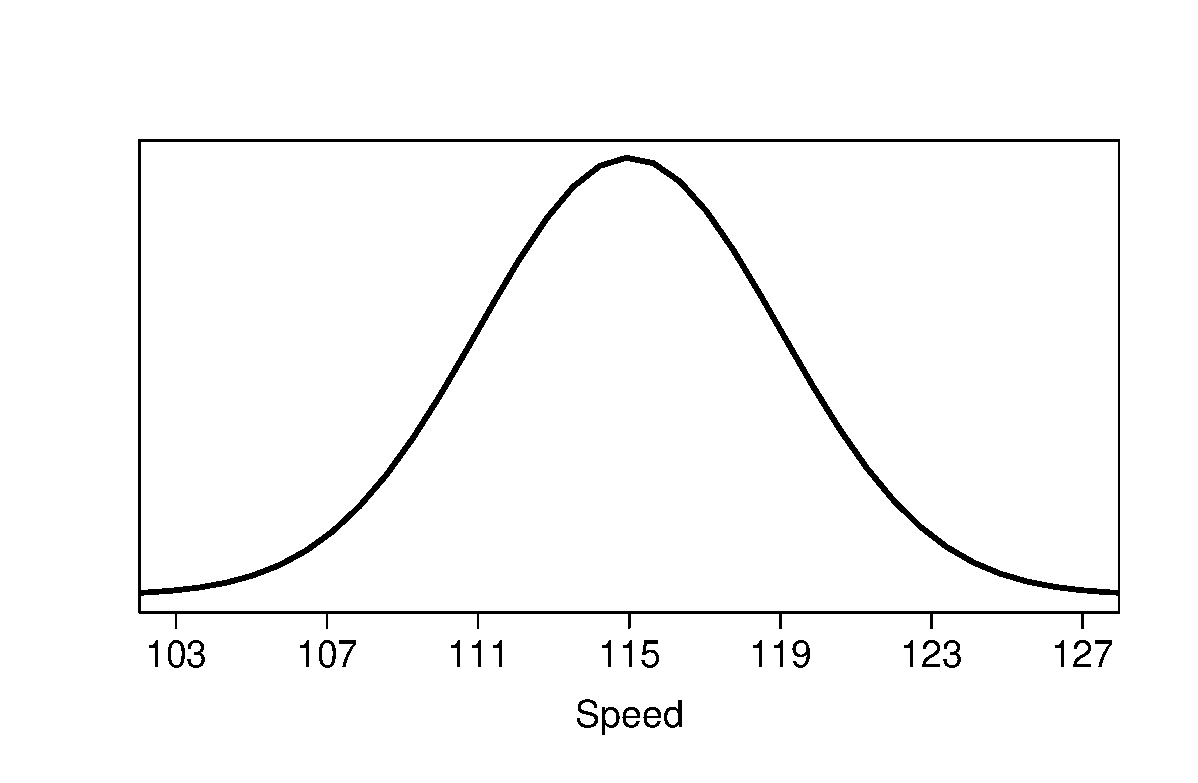
\includegraphics[width=0.9\textwidth, trim = 1.5cm 0.5cm 1cm 1.5cm, clip]{NormSpeed}
\end{tabular}
\item \quad\\[-1.45cm]
\begin{align*}
\Pr(X > 120) = \Pr(Z > \tfrac{120-115}{4}) &= \Pr(Z > 1.25) \\
&= 0.1056
\end{align*}
\item \quad\\[-1.45cm]
\begin{align*}
\Pr(X < 100) = \Pr(Z < \tfrac{100-115}{4})& = \Pr(Z <  -3.75) \\
&= \Pr(Z > 3.75) \\
&= 0.000088.
\end{align*}
\end{enumerate}
\end{minipage}\hspace{0.04\textwidth}
\begin{minipage}[t]{0.47\textwidth}
\quad\\[-1cm]
\begin{enumerate}
\item[d)] \quad\\[-1.45cm]
\begin{align*}
\Pr(100 &< \,X < 110) \\
&= \Pr(X > 100) - \Pr(X > 110)\\
&=\Pr(Z > \tfrac{100-115}{4}) - \Pr(Z > \tfrac{110-115}{4}) \\
&=\Pr(Z > -3.75) - \Pr(Z > -1.25) \\
&=\Pr(Z < 3.75) - \Pr(Z < 1.25) \\
&= (1 - 0.000088) - (1-0.1056)\\
&=  0.999912 - 0.8944\\
&= 0.1055.
\end{align*}
\item[e)] \quad\\[-1.45cm]
\begin{align*}
\Pr(X > x) &= 0.01 \\
\Pr(Z > \tfrac{x-115}{4}) &= 0.01 \\[0.2cm]
\text{From tables: } \Pr(Z > 2.33) &= 0.0099 \approx 0.1 \\[0.2cm]
\Rightarrow \frac{x-115}{4} &= 2.33 \\
\frac{x-115}{4} &= 2.33 \\
x-115 &= 2.33(4) \\
x &= 115 +2.33(4) \\
x &=  124.32.
\end{align*}
\end{enumerate}
\end{minipage}
\end{minipage}}\vspace{0.03\textwidth}





\framebox[1.02\textwidth]{
\begin{minipage}[t]{0.98\textwidth}
\begin{minipage}[t]{0.47\textwidth}
\subsection*{Question 7}
\begin{enumerate}[a)]
\item\quad\\[-1.45cm]
\begin{align*}
\Pr(\mu - 3 \sigma &< \,X < \mu + 3 \sigma) \\
&= \Pr(X > \mu - 3 \sigma) - \Pr(X > \mu + 3 \sigma)\\
&=\Pr(Z > \tfrac{\mu - 3 \sigma - \mu}{\sigma}) - \Pr(Z > \tfrac{\mu + 3 \sigma - \mu}{\sigma}) \\
&=\Pr(Z > -3) - \Pr(Z > 3) \\
&=\Pr(Z < 3) - \Pr(Z > 3) \\
&=1 - \Pr(Z > 3) - \Pr(Z > 3) \\
&=1 - 2\,\Pr(Z > 3) \\
&=1 - 2(0.00135) \\
&=  0.9973.
\end{align*}
\item Note that the workings are the same as in part (a) above except that we have $k$ instead of $3$.
\begin{align*}
\Pr(\mu - k \sigma < \,X < \mu + k \sigma) &= 0.95 \\
&\vdots\\
\Rightarrow 1 - 2\,\Pr(Z > k) &= 0.95 \\
- 2\,\Pr(Z > k) &= -1 + 0.95 \\
2\,\Pr(Z > k) &= 1 - 0.95 \\
\Pr(Z > k) &= \frac{1 - 0.95}{2} \\
\Pr(Z > k) &= 0.025 \\[0.4cm]
\Rightarrow k &= 1.96.
\end{align*}
\end{enumerate}
\end{minipage}\hspace{0.04\textwidth}
\begin{minipage}[t]{0.47\textwidth}
\quad\\[-1cm]
\begin{enumerate}
\item[c)] This is the same as part (b) except we have 0.99 rather than 0.95.
\begin{align*}
&\vdots\\
\Rightarrow \Pr(Z > k) &= \frac{1 - 0.99}{2} = 0.005\\[0.4cm]
\Rightarrow k &= 2.58.
\end{align*}
\item[d)]\quad\\[-1.45cm]
\begin{align*}
\Pr(X > \mu + 1.64 \sigma)
&=\Pr(Z > \tfrac{\mu + 1.64 \sigma - \mu}{\sigma})\\
&=\Pr(Z > 1.64) \\
&= 0.0495 \approx 0.05.\\
\end{align*}
\end{enumerate}
\end{minipage}
\end{minipage}}\vspace{0.03\textwidth}











\end{document} 